%%%%%%%%%%%%%%%%%%%%%%%%%%%%%%%%%%%%%%%%%%%%%%%
%%%		Title:			faq4u.tex
%%%		Author:			Kevin Bergman
%%%		Created:		29/07/2014
%%%		Last edit:		01/08/2014
%%%%%%%%%%%%%%%%%%%%%%%%%%%%%%%%%%%%%%%%%%%%%%%


\documentclass[letterpaper,10pt,titlepage,fleqn]{article}
\setlength{\mathindent}{1cm}

\usepackage{graphicx}
\usepackage{listings}
\usepackage{amssymb}
\usepackage{amsmath}
\usepackage{amsthm}
\usepackage{alltt}
\usepackage{float}
\usepackage{color}
\usepackage{url}
\usepackage{balance}
\usepackage[TABBOTCAP, tight]{subfigure}
\usepackage{enumitem}
\usepackage{pstricks, pst-node}
\usepackage{geometry}
\usepackage{hyperref}
\usepackage{textcomp}
\usepackage{listings}

\geometry{textheight=9in, textwidth=6.5in}
\newcommand{\cred}[1]{{\color{red}#1}}
\newcommand{\cblue}[1]{{\color{blue}#1}}

\def\name{Kevin Bergman}

\hypersetup{
  colorlinks = true,
  urlcolor = black,
  pdfauthor = {\name},
  pdfkeywords = {},
  pdftitle = {},
  pdfsubject = {F.A.Q.},
  pdfpagemode = UseNone
}

\parindent = 0.0 in
\parskip = 0.2 in

%\titlehead{\centering
\includegraphics{images/kelley1.eps}}
\title{F.A.Q. for CS162 at Oregon State University}
% \author{Kevin Bergman}
\date{\today}


\begin{document}
\begin{titlepage}
    \centering
    \vfill
    {\bfseries\Large
		F.A.Q. for CS162 at Oregon State University
        \vskip2cm
		\date{\today}

	}    
    \vfill
     
\includegraphics[width=15cm]{images/kelley1.eps} % also works with logo.pdf
    %  
\includegraphics[width=15cm]{images/kelley2.eps} % also works with logo.pdf
    %   
\includegraphics[width=15cm]{images/kelley3.eps} % also works with logo.pdf
    %  \includegraphics[width=15cm]{images/kelley4.eps} % also works with logo.pdf
    %  
\includegraphics[width=15cm]{images/kelley5.eps} % also works with logo.pdf
    \vfill
    \vfill
\end{titlepage}


%\maketitle

%\begin{figure}[ht!]
%  
\includegraphics[scale=0.5]{images/kelley1.eps}
%  
\includegraphics[scale=0.5]{kelley2.eps}
%  
\includegraphics[scale=0.5]{kelley3.eps}
%  \includegraphics[scale=0.5]{kelley4.eps}
%  
\includegraphics[scale=0.5]{kelley5.eps}
%  \includegraphics[scale=0.5]{kelley6.eps}
%\end{figure}





\tableofcontents

\newpage

\section{Intro}
This is a simple guide for CS162, but would be useful for those in 160 or 161
as well. It was created by a TA who over time noticed several repeating and
common questions from his students, and got tired of endlessly explaining the
concepts. Hopefully this guide will stand the test of time, serving well those
who review it. It is written in LaTeX and the source is available on Github: 
https://github.com/el7/faq4u. This is done so that after myself has left the
schooling system, that another TA may pick it up and update any changes that
come to play. It's meant to be a living document for the university. Though some
items in the document may change, several will likely stay the same. Enjoy.

It should be noted that your instructor may make some of these requirements and 
failing to use them could mean point deduction. For instance, if your code is
unreadable without any comments, or if you have an excessive amount of files
without a makefile. Just don’t make grading hard for us.




\section{Web Portals}


\subsection{TEACH}
https://secure.engr.oregonstate.edu:8000/teach.php?type=want\_auth

This is a web portal to a server on campus where we collect your submissions. Each
time you submit to TEACH, a new folder is created titled with your username in a
 parent folder cooresponding to the assignment. If you submit to TEACH more than once, the folders
on our end get renamed as so:

\begin{tabbing}
\hspace*{2cm}\=\hspace*{3cm}\= \kill
username/ 		\>\> Most recent submission. \\
username.old.1/ \>\> Very first submission. \\
username.old.2/ \>\> Second submission, etc. \\
\end{tabbing}

Keep in mind: It’s a general principle to always include all of your work every
time you submit. Don’t split up the files in the submissions. For instance if
your professor asks you to submit a writeup before the actual assignment, you'll
want to first submit the writeup, and then include it again once you submit the
code. Unless otherwise specified, we will likely look over your .old folders.


\subsection{Canvas}
Coming soon to OSU. This will supposedly replace Blackboard in Fall 2014. 


\subsection{Blackboard}
https://my.oregonstate.edu/webapps/portal/frameset.jsp

eCampus interface. It has your grades, holds a lot of course material, and you
take tests and quizzes here. There’s also a discussion forum that is sometimes
used.


\subsection{Piazza}
https://piazza.com/

Discussion board, used by many professors.


\section{Submission}
* Also see Web Portals

Though compeltely dependant on the class and professor, I've found Assignments
are generally due at 23:59:59 the night of the due date. Depending on how the
professor sets up their submission system, you might not be able to submit
anything after the time is up- making you email your work to a TA. Similarly with online quizzes
and exams. 



\subsection{Source Files}
\subsubsection{file.cpp}
These are the C++ source files you will be working with. Each program submission
will (likely) have at least one of these, if not many.


\subsubsection{file.h / file.hpp}
These are header files, which is a supporting file to the source files. You
don't necessarily need these in your assignments (unless the instructor asks for
them), but they can be beneficial. For instance they can make your code and project
more readable, and are essential in good program design. The biggest difference
between .h and .hpp files is that the .hpp file extension should indicate to the
user that the file is not interchangeable with a C program, whereas .h could be.


\subsection{Writeup}
This is a PDF document you will include with all (most) submissions.
These are the generally required sections, but will vary depending on your
instructor or the particular assignment:

\begin{tabbing}
\hspace*{2cm}\=\hspace*{3cm}\= \kill
Requirements: 	\>\>Talk about the assignment requirements. \\
Assumptions: 	\>\>Is there something that’s not clear? \\
Design: 		\>\>How do you envision your program? \\
Testing:		\>\>Test valid and invalid values. What is observed? \\
Reflection: 	\>\>Discuss your project in retrospect. \\
\end{tabbing}


\subsubsection{Design \& Testing}
These are usually two of the most important sections of the writeup. The design
is supposed to reflect your conception of the program.

Testing is supposed to reflect the idea that you've used your program and
understand what happens when you use it with interesting values. Generally this
section is just a table with at minimum three columns: Input, Expected Output,
Actual Output. Then the rows consist of various input you've given your program.
You'll want to test obvious cases (1, 5, 8), boundary cases (0, 10, 100), and
extreme cases (999999, negative numbers). The previous numbers are arbitrary and
depend on your program, but hopefully you get the idea. You then record this
data under the testing section of the writeup.


\subsection{Makefiles}
You can think of makefiles as an engine to start your engine. The
file has a special language with semantics meant for build control. During your
162 adventures many of you will make programs that require 10 or more files,
making compilation confusing, difficult or tedius. That is where makefiles come
in handy. When you have a working makefile alongside your project, you can turn
this compilation command:
\newline
\newline
g++ -std=c++0x driver.cpp class1.cpp class1.hpp class2.cpp class2.hpp
other\_class.cpp other\_class.hpp parent\_class.cpp parent\_class.hpp
child\_class.cpp child\_class.hpp -o p1
\newline
\newline
To this:
\newline
\newline
make
\newline

Much easier! There should be two makefiles included somewhere alongside this document; a simple
makefile that's easy to understand, and a more robust makefile that's more
reusable. Please include a makefile in your submissions. 


\subsection{Archiving}
Please archive your work. If you don't understand the importance of this, let me
tell a story. I was grading an assignment one term that dealt with file IO. The
student had (I'll assume accidentally) made a program that deleted some of their
header files and an input.txt file after the first execution. They didn't
archvie their work before submission and so the files were lost and they
recieved a poor grade. Had they submitted an archive, I would have been able to
just pull their work back out of the archive. Let their lesson be your own:
archive you work. 

For compatability reasons, Zip is the perferred method. This is because it's
naturally supported on all the big operating systems. Alternatively, your TA may
request another tool. 

This is how the archive should be named:\\
\textbf{class\_assignment\_username.extension}\\\\
Example:\\
\textbf{cs162\_assignment3\_cooljoe.zip}

\section{SSH and the Campus Server}

As a TA or instructor, we are responsible for grading your
material. As you might imagine there are an anbsurd amount of ways to code,
compile, and run programs. However for our convinience, we're going to be
grading you based on how your programs work on the school's server. This means
it's completely within your benifit to at least test your work there before
submitting, or as I would suggest, just learn to develop your programs there.
I'll give a short guide to getting to the server.

Windows: Use PuTTY or KiTTY

\begin{figure}[ht!]
  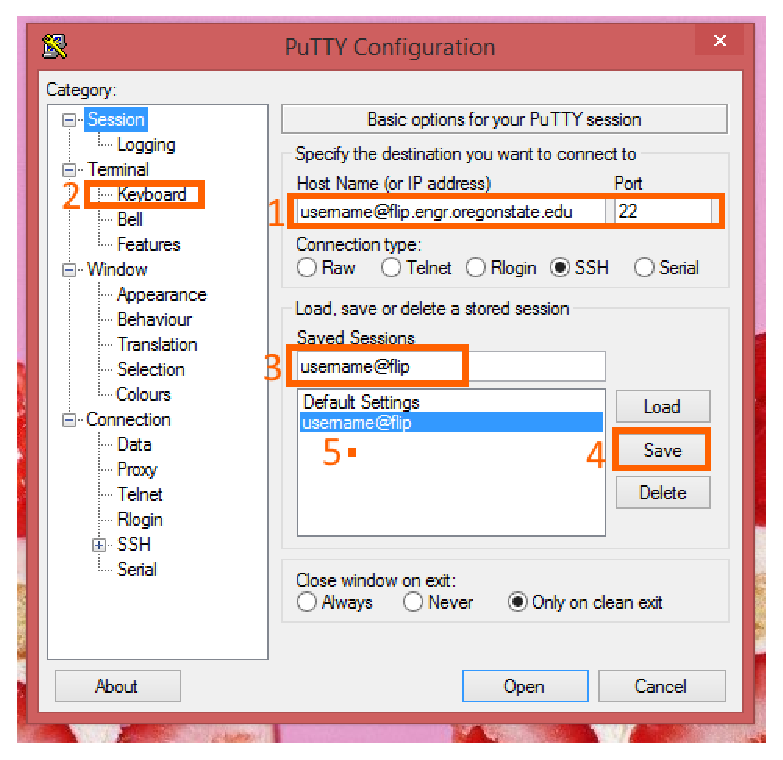
\includegraphics[scale=0.5]{images/putty1.eps}
  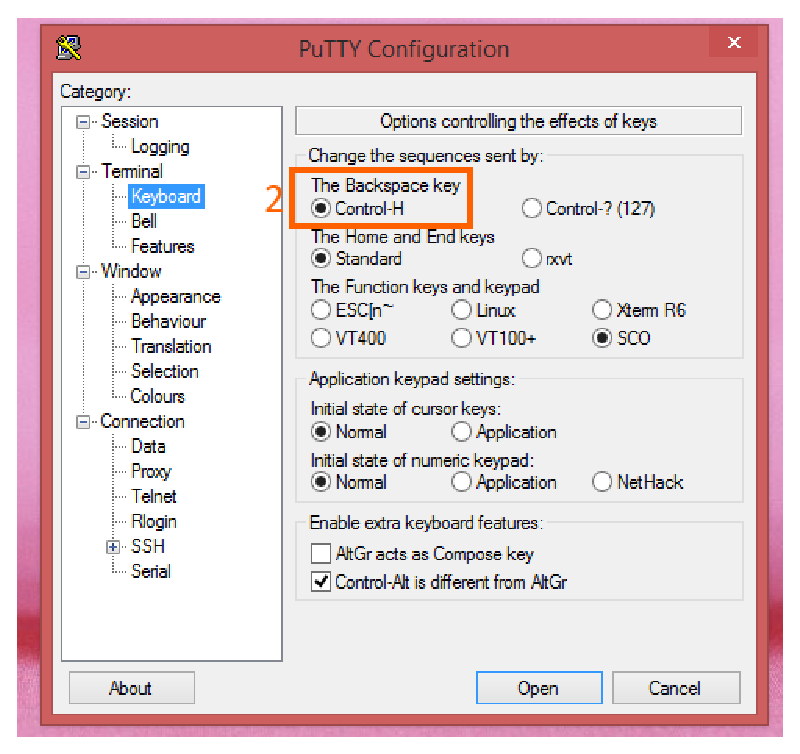
\includegraphics[scale=0.5]{images/putty2.eps}
\end{figure}

\textbf{1.} Enter your username and the server's address. Note: port 22 is standard.
\textbf{2.} Go to the keyboard settings. Make sure Control-H is set for backspace.
\textbf{3.} Enter a profile name. I usually use the username and server name.
\textbf{4.} Save the profile. Do this after making the above changes.
\textbf{5.} Double click the profile to load it. 

Linux / Mac: Use a terminal program.

\begin{figure}[ht!]
  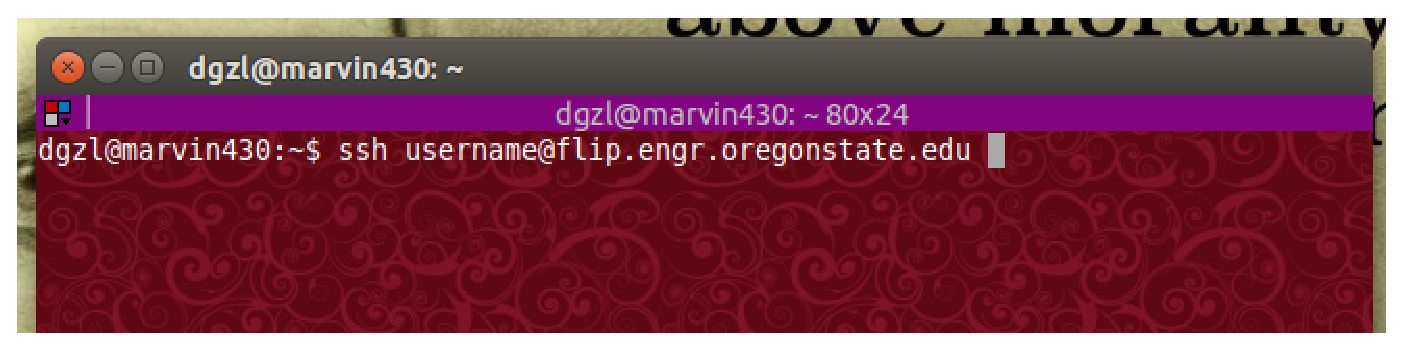
\includegraphics[scale=0.5]{images/ssh_terminal.eps}
\end{figure}    

\textbf{1.} Enter 'ssh username@address' into the terminal and press enter.


\begin{figure}[ht!]
  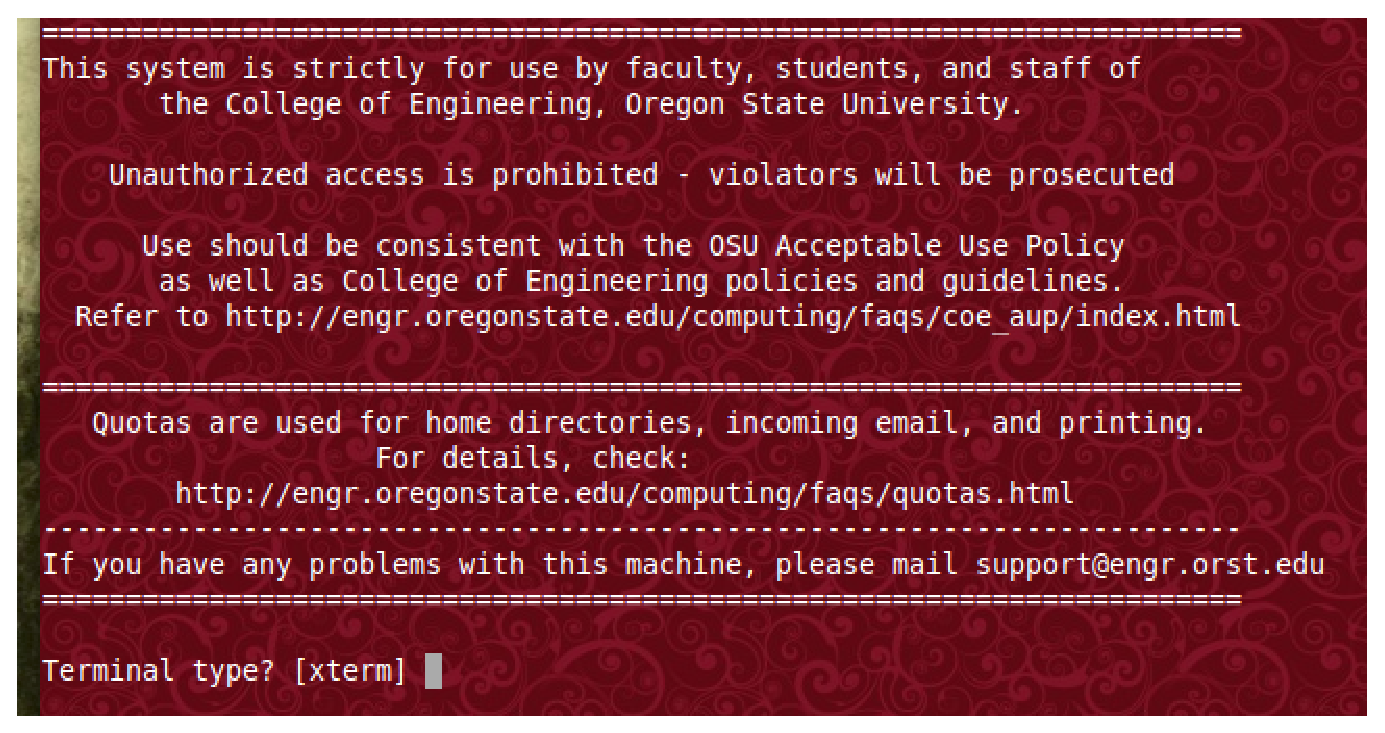
\includegraphics[scale=0.5]{images/ssh_terminal2.eps}
\end{figure}    

This is the MOTD, it's asking what kind of terminal you want. Just press enter..

\newpage
\newpage

\section{Basic Shell Commands}

Since your programs must work on the school servers, and since many of your future
CS classes will require Linux knowledge, it's a good idea for you to learn some
basic shell commands. Nothing fancy, just getting around.


\begin{tabbing}
\hspace*{2cm}\=\hspace*{3cm}\= \kill
pwd									\>\>Prints the current working directory.\\
ls									\>\>Lists files in current directory.\\
ls -a								\>\>Includes self and parent folders, and hidden files\\
ls -l								\>\>Shows permissions, timestamps, groups, etc.\\
mkdir newdir						\>\>Creates new folder.\\
cp file1.cpp file2.cpp				\>\>makes a copy of file1 and names it file2.\\
cd newdir/							\>\>change directory to nested folder2\\
									\>\>( relative path )\\
cd ~/folder1/						\>\>change directory to folder1.\\
									\>\>( absolute path, ~/ is your home folder )\\
cd ../								\>\>change directory to the parent folder\\
									\>\>( ../ is a link the the parent folder )\\
rm file1 file2.c file3.cpp			\>\>removes these files.\\
rm -r folder1/						\>\>removes folder and everything in it.\\
mv file1.cpp ../folder2/			\>\>moves a file to different folder.\\
mv file1.cpp file2.cpp				\>\>keep file in same folder but renames it.\\
man ascii							\>\>Man page (and tables) for the ASCII character set.\\
man man								\>\>Gives the manual page for the man command.\\
top									\>\>Lists working processes in resource-heavy order.\\
exit								\>\>An explicit exit from a terminal (or ssh
session). \\
\end{tabbing}

\begin{figure}[ht!]
  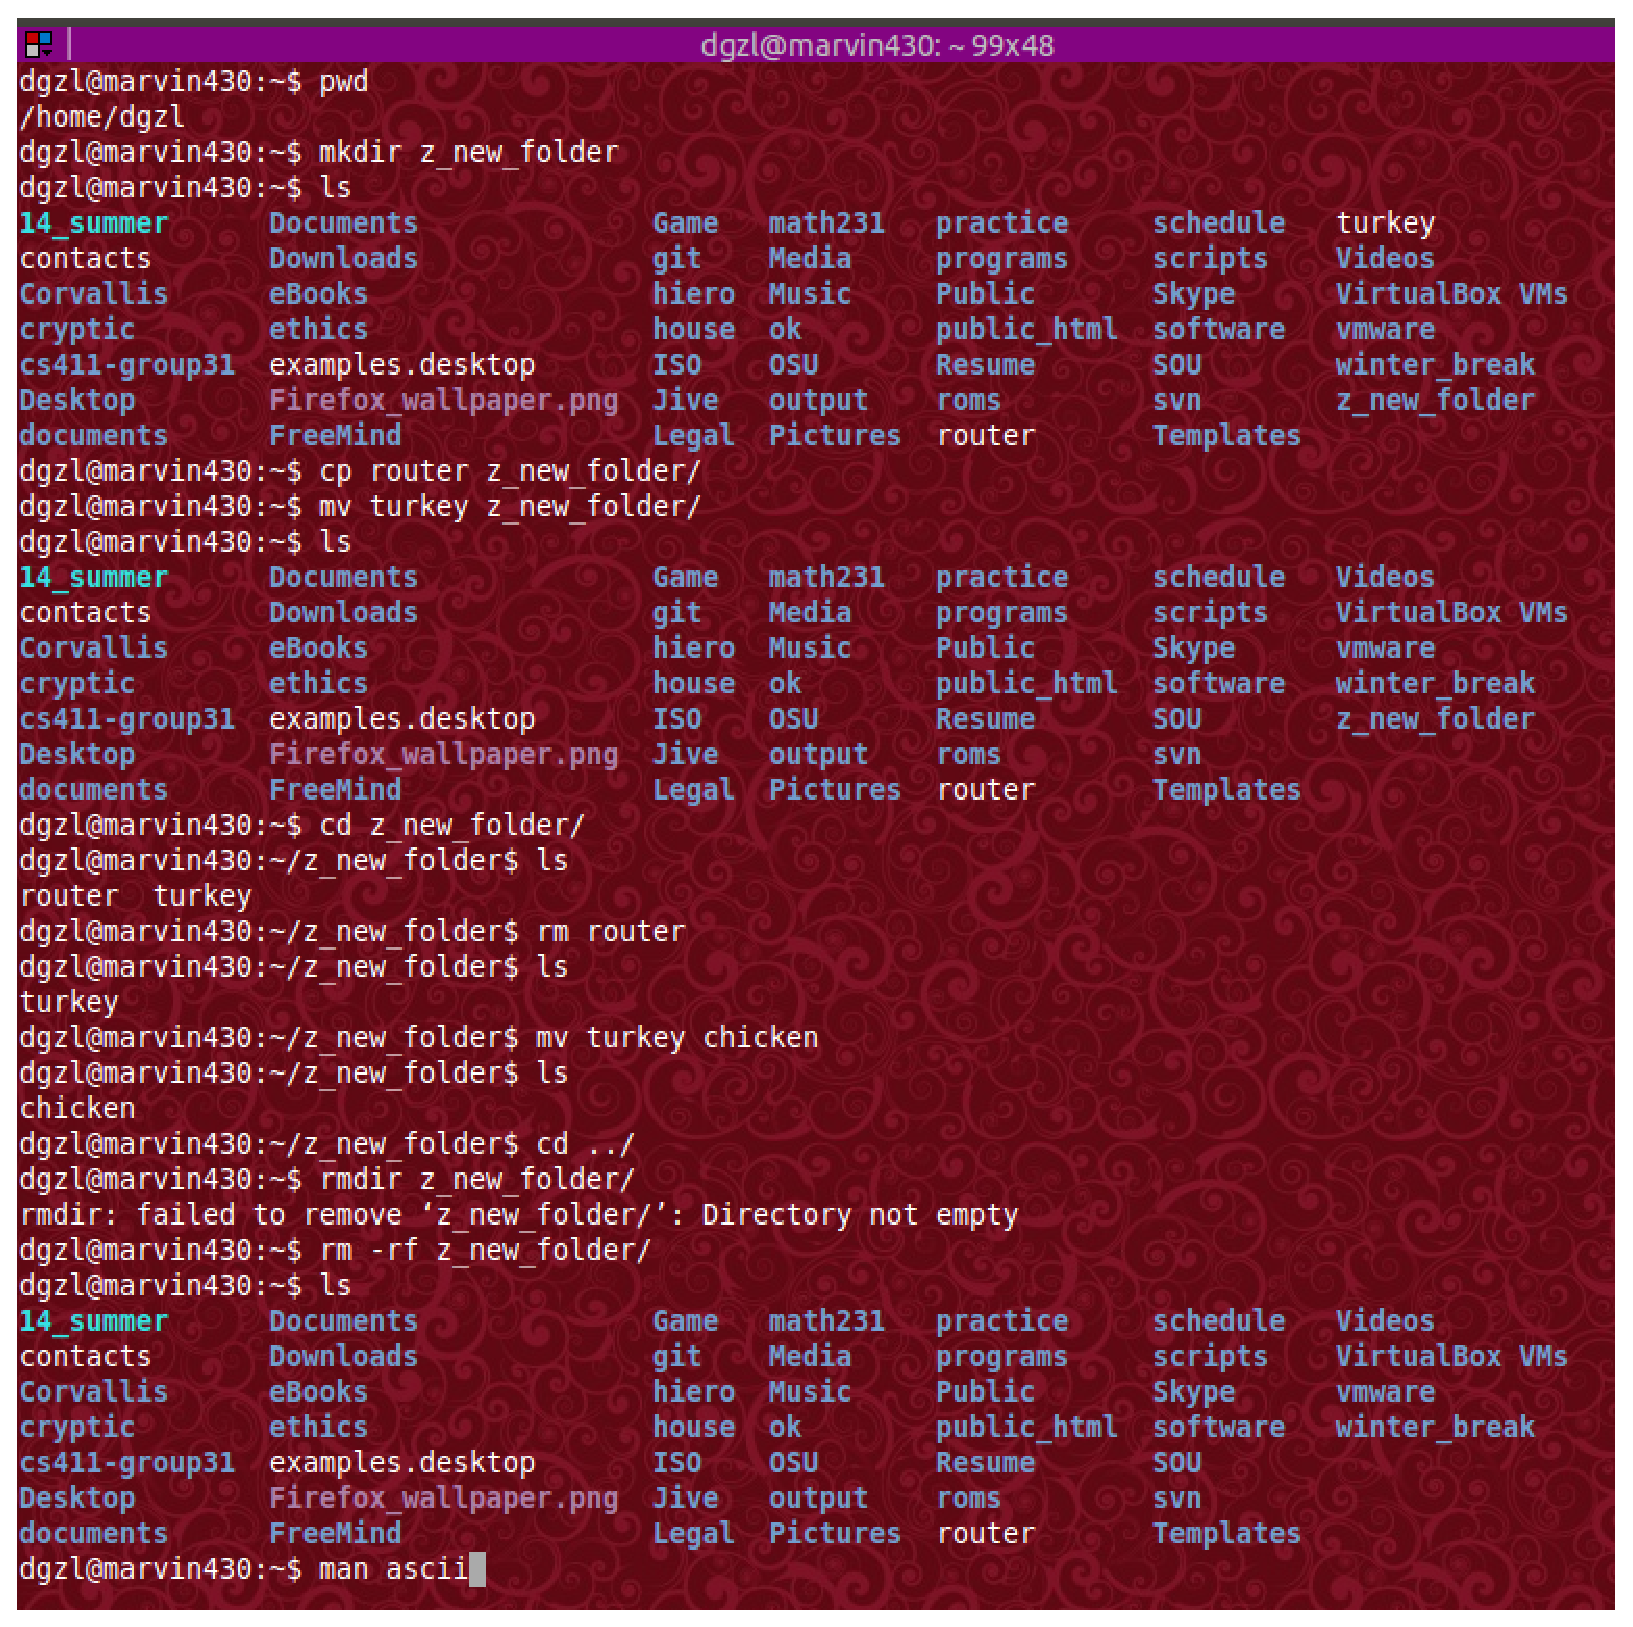
\includegraphics[scale=0.5]{images/shell_commands.eps}
\end{figure}

First \textbf{pwd} is used to print the working directory. Then \textbf{mkdir}
is used to make the new directory 'z\_new\_folder'. \textbf{ls} is then used to
print the contents of the current directory. You can see 'z\_new\_folder' at the
end. Then we used \textbf{cp} to copy the file 'router' to the new folder, and
used \textbf{mv} to move the file 'turkey' to the new folder. We then print out
the directory again, and you can see the file 'turkey' is no longer there. We
then use \textbf{cd} to move into the new folder, and print out it's contents.
You can see the 'router' and 'turkey' files. We then use \textbf{rm} to remove
the 'router' file. Then we use \textbf{mv} on 'turkey' again, but instead of 
moving it we are renaming it 'chicken'. We then use \textbf{cd ../} to move back
a folder, and try to use \textbf{rmdir} on the new folder. We get an error
saying we can't remove it because there are items inside it. Since I know
there's nothing important in there, I use \textbf{rm -rf} to remove the folder.
The -r option tells the program to search and delete things recursivly, and -f
means to use force (don't ask permission). Finally, \textbf{man} is short for
'manual' and lets you see manual pagest for certain things. This example shows
the manual page for the ascii character set. Give it a try.


\section{Useful CLI Tools}
ssh. This tools lets you connect your host computer to a remote terminal.

example:
ssh username@flip.engr.oregonstate.edu

sftp. It’s like using SSH but with easy file transferring commands. Adding ‘l’
in front of the command applies the command to the host computer. 
example:
sftp username@flip.engr.oregonstate.edu    connects to the flip server.
ls                        Lists files on remote server.\\
lls                        Lists files on host server\\
cd dir/                        Changes directories on remote server.\\
lcd dir/                        Changes directories on host server.\\
put file.cpp                    Transfers file from host to remote server.\\
get file.cpp                    Transfers file from remote to host server.\\
\\ 
tar. It's an archiving / compression tool used widely in *nix.

Compress
tar cvjf cs162\_assignment2\_username.tar.bz2 file1.cpp file2.cpp file3.cpp

Decompress
tar xvjf cs162\_assignment2\_username.tar.bz2

cvjf are options: 
c / x:		(create / xtract) archive
v:			verbose, 
j:			bzip2 compression, 
f:			use the following file.

cs162\_assignment2\_username.tar.bz2 is the name of the compressed file we’re
going to create. file1.cpp, file2.cpp, file3.cpp are the files that are going to
be archived.    \\
\\
alias. This tool lets you make custom command line commands. \\
example:\\
alias                                Lists all current aliases. \\
alias l=’ls’                            Binds ‘l’ to ls.\\
alias flip=’ssh username@flip.engr.oregonstate.edu’        Binds ‘flip’ to ssh\\
to flip server.\\

grep. Lets say you want to look for a particular bit of text, but you have
several files to search through. Wouldn’t be efficient to open each of them and
search, would it? Grep comes in handy by scanning as many files as you like for
text.\\
example:\\
grep ‘text’ *			This searching the term 'text' in all (*) of the files
in the folder.\\


find. Like grep but used for file names.\\

vim/emacs.  Command line text editor that comes stock on all (most) Linux
distributions. I encourage you to learn one and use this throughout your
courses. Benefits include increased code dexterity, more exposure to the CLI,
and they’re stock on nearly every unix environment, so you can edit files on an
ssh connection. \\
\\
A short guide to Vim:\\
\\
If you use your keyboard’s Delete command, it saves the deleted character into a
register.\\

There is a file saved in your home folder that is used for your vim
configurations. The file (.vimrc) can be used to customize your vim experience.
Here is an example .vimrc file: <link to rc>\\

Useful Vim commands: \\
\\
:w: save file\\
:q: quit editor\\
:q!: quit without saving\\
:wq: Save and quit\\
\\
Movement:\\
(same as arrow keys)\\
h: left\\
j: down\\
k: up\\
l: right\\
0: Move to first character of the line. Same as <Home>.\\
\$: Move to the last char of the line. Same as <End>.\\
\#<direction>: Move \# units in <direction>.\\
\\
i (when in command mode): change to insert mode.\\
esc (when in insert mode): change to command mode.\\
(the following will assume we are in command mode)\\
yy: yank (copy) the current line.\\
dd: delete (and copy) the current line.\\
y<arrow> (where <arrow> is an up / down directional key): yank the current line\\
and 1 line in that direction.\\
d<arrow> (where <arrow> is an up / down directional key): delete (and copy) the\\
current line and 1 line in that direction.\\
y\#<arrow> (where <arrow> is an up / down directional key and <\#> is a number
greater than 0): yank the current line and \# lines in that direction.
d\#<arrow> (where <arrow> is an up / down directional key and <\#> is a number
greater than 0): delete (and copy) the current line and \# lines in that
direction.\\
p: Paste the most recent item in the save register. \\
u: Undo.\\
<ctrl>R: Redo.\\
v: visual mode, similar to highlighting with a mouse. Can be used with other
commands like y and d.\\
x: Deletes the character in front of the cursor. Same as using the <delete>
button.\\
ZZ: Save and quit, like :wq but can be done easily with one hand.\\
ZQ: Quit and exit, like :q!.\\
gg=G: This will use Vim’s auto-indent feature. It comes in handy if you have a
particularly messy coding style.\\
/<string> (where <string> is a string of your choice): This will search your
program for and highlight <string>.\\
n: Moves your cursor to the next instance of the term you searched for.\\
N: Moves your cursor to the prev instance of the term you searched for. \\
:\%s/string1/string2/gc: This is a search and replace command where string1 is
your string to replace and string2 is the string to replace it with. The ‘c’ at
the end of this command means to ask you permission before overwriting at each
instance. Without the ‘c’ it will not ask.\\
:set number: Shows / hides line numbers.\\
:<number>: Jumps to that line number.\\
:set colorscheme <scheme>: Changes text colors based on <scheme>. \\
*: Highlights and searches for whatever text your cursor is on.\\
\\
\\

\section{Style Guide}
Code should look nice. 
It should have logical and consistent Indentation. 
There should be descriptive yet concise comments describing the functions. If
your code is sloppy you may recieve comments from your TA or even point
deductions.

See style guide document?


\section{Useful Software}
FileZilla. A file transfer protocol (FTP) program. Used for transferring files
to / from another computer. \\

PuTTy (alt: KiTTy). Secure Shell (SSH) software for Windows. It gives you a
linux terminal from OSU’s “Flip” sever. Don’t forget to change keyboard settings
to “Alt-H” so you can use backspace. \\

GIT / SVN \\
Revision control software. This is beyond the scope of these classes, but
they’re very useful to learn and you will need it in future classes / work.\\

Vim (alt: Emacs).
Advanced command line text editor.

Notepad++


\section{Useful Websites}

github.com\\
pastebin.com\\
stackoverflow.com\\
cplusplus.com\\
linuxquestions.com\\
piazza.com\\
blackboard.com\\
\\

\section{Other}


\section{nothing of importance}

This section is for testing and will be deleted before released.

\begin{lstlisting}[frame=trBL]
Code block
\end{lstlisting}

\lstset{backgroundcolor=\color{yellow}}
\begin{lstlisting}[frame=single, framerule=0pt]
Code block
\end{lstlisting}

\end{document}
